% beamer + fontspec + TikZ + pgfplots + hyperref + graphicx
\documentclass{beamer}
\usetheme{Madrid}
\usepackage{fontspec}
\setsansfont{texgyreheros}[Extension=.otf, UprightFont=*-regular, BoldFont=*-bold, ItalicFont=*-italic, BoldItalicFont=*-bolditalic]
\usepackage{tikz}
\usetikzlibrary{arrows.meta,positioning}
\usepackage{pgfplots}
\pgfplotsset{compat=1.18}
\title{Plots and Pictures}
\author{A. Speaker}
\date{2026}
\begin{document}
\frame{\titlepage}
\begin{frame}{A diagram}

\begin{tikzpicture}[node distance=2cm, every node/.style={draw,rounded corners}]
\node (a) {Source}; \node[right=of a] (b) {Engine}; \node[right=of b] (c) {PDF};
\draw[-Stealth] (a) -- (b); \draw[-Stealth] (b) -- (c);
\end{tikzpicture}
\end{frame}
\begin{frame}{A plot}
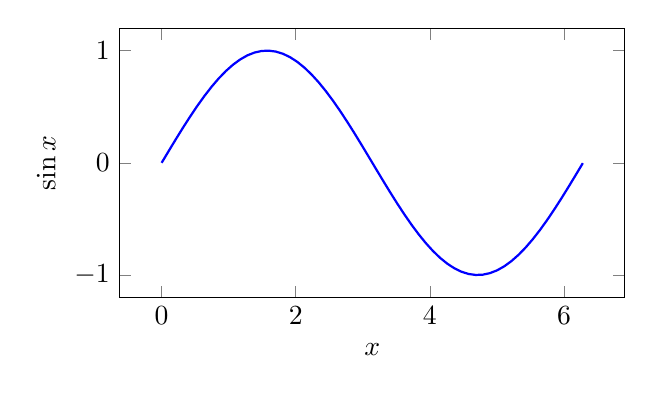
\begin{tikzpicture}
\begin{axis}[width=8cm,height=5cm,xlabel=$x$,ylabel=$\sin x$]
\addplot[domain=0:6.28,samples=60,blue,thick]{sin(deg(x))};
\end{axis}
\end{tikzpicture}
\end{frame}
\begin{frame}{An image and a link}
\includegraphics[width=4cm]{example-image-a}\hfill
\href{https://www.ctan.org}{CTAN}.
\end{frame}
\end{document}
